\chapter{基于南极的天文数据观测与处理} \label{chapter:obs_red}

\section{南极天文背景} \label{sec:antarticabg}

搜索系外行星需要长时间基线和高精度的天文观测,然而因为地球在做周日自转并且存在大气包层,
因而在地球上很难同时满足这些严苛的观测条件。\S \ref{sec:transit} 中曾提到空间望远镜 CoRoT
\cite{Bargeetal2008CoRoT} 与 $Kepler$\cite{Boruckietal2010},它们花费了昂贵的代价(数十亿
美元)才能得到满足上述观测条件的数据,事实证明它们也取得了令人瞠目的科学成果。而横向对比,
南极台址(Antarctic plateau)作为理想的地面台址可在经费花费相对较少的同时,依然拥有良好的
观测条件 --- 而这得归功于以下几点优势:

\begin{itemize} %\setlength{\itemindent}{0.3in}
\item[--] 南极高台地址拥有大陆上最冰冷、干燥\footnote{以绝对水气值来衡量。}的空气(文献\citen{Burton2010} )。此气候条件尤为适合进行光学、红外以及亚毫米波段的天文观测\cite{Lawrence2004}。
\item[--] 南极高台水平高度高,因而空气层厚度薄,大气湍流少,空气状况也更稳定\cite{Bonner2010}。
\item[--] 极夜(Polar nights)为观测提供了长达 3 个月的连续观测条件,这也是观测系外行星最重要的优势\cite{Rauer2008}。
\end{itemize}

\begin{figure}[t]
\centering
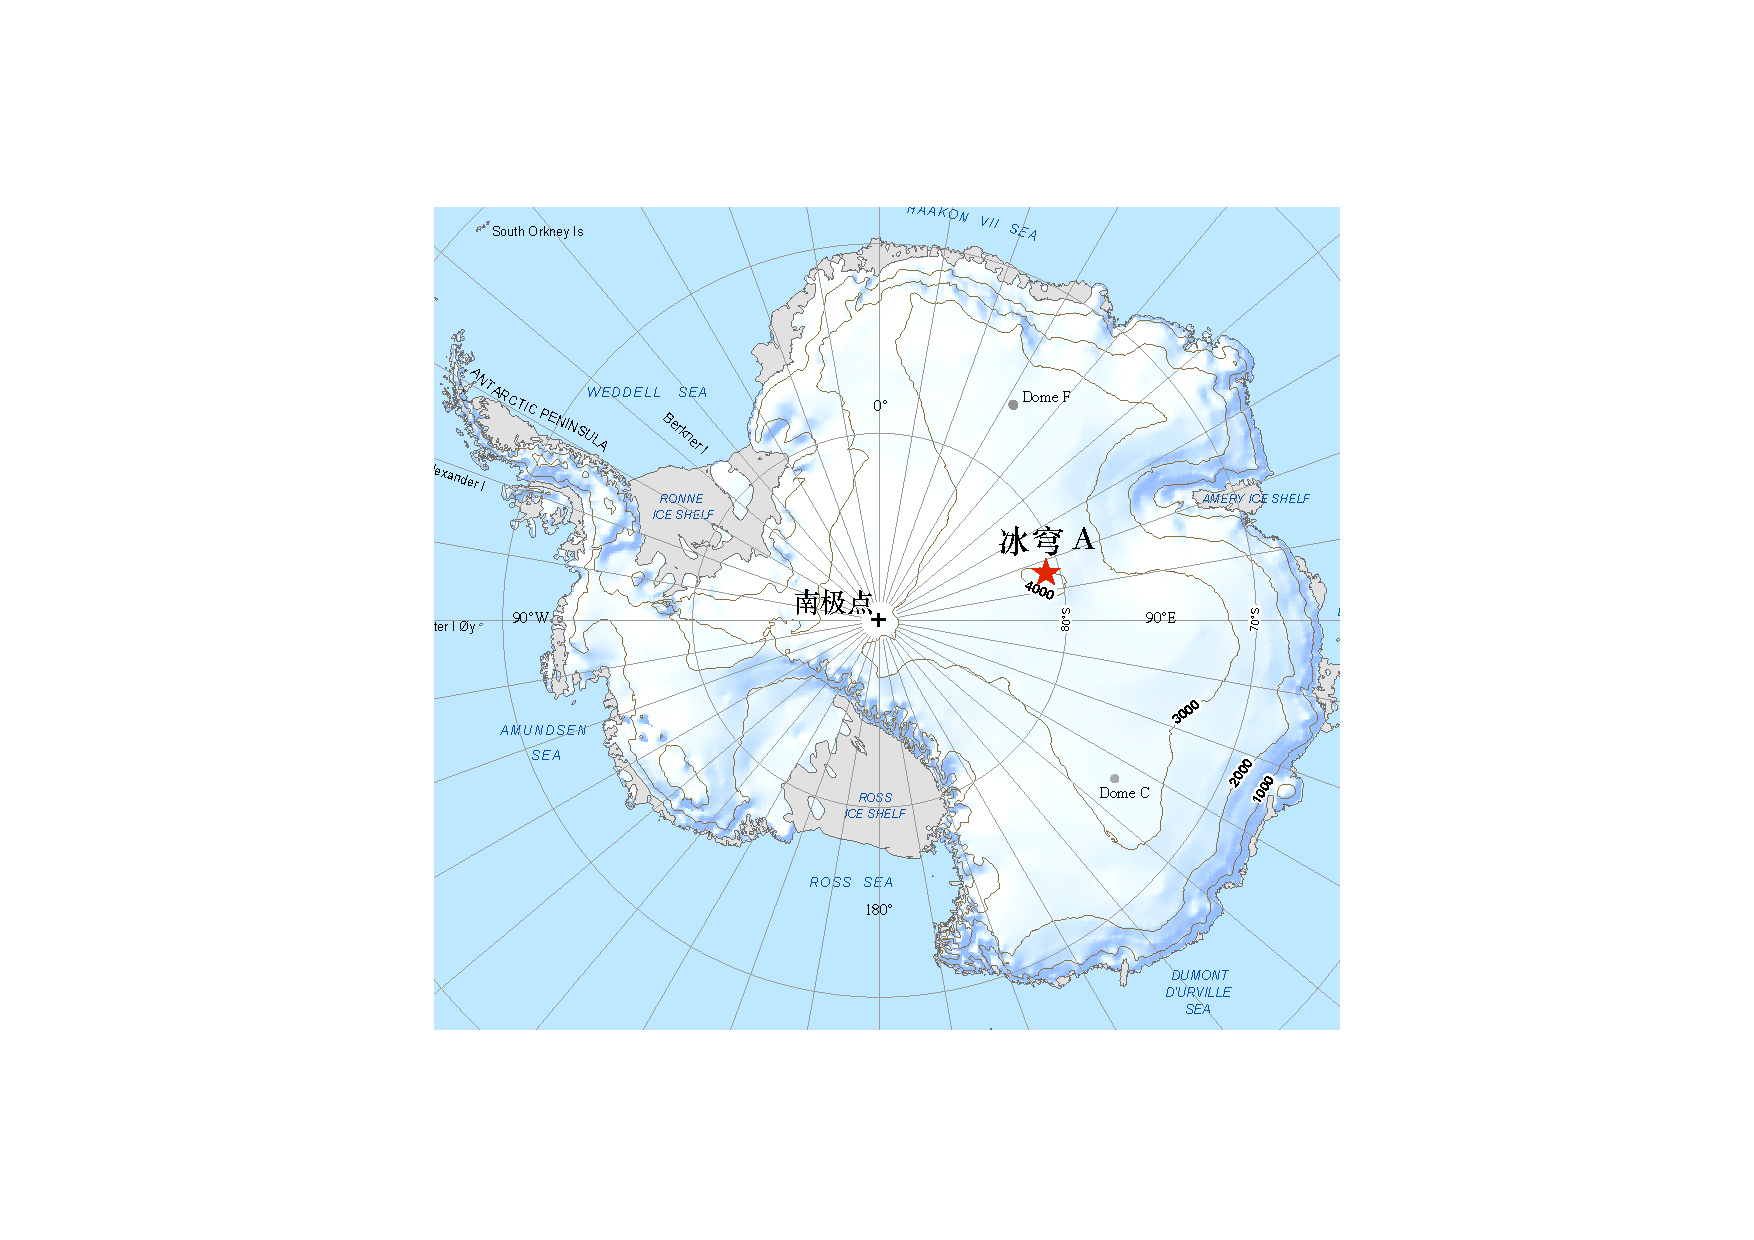
\includegraphics[width=1.0\textwidth]{figures/chapter2/f1_DomeA.pdf}
\caption{南极地理位置图,暗咖啡色曲线表示地形等高线。可以看到冰穹 A 台址(中国,以红星标注)位于南极大陆最高点,另外冰穹 C(澳洲) 和 F(日本)分别以灰色圆点表示。此地图版权 Australian Antarctic Division。}
\label{fig:domeasite}
\end{figure}

得益于拥有如此得天独厚的先天条件,南极台址在短短 30 年内就已吸引了大批的天文开拓实验与项目
(南极天文的历史相关细节请查阅综述文献\citen{Indermuehle2005})。Grec 等人于 1980 年开启首个
地处南极的光学实验\cite{Grec1980}。随后一大批天文学成果相继涌现\cite{Burton2010},以高精度测光
科学为例:ASTEP(Antarctic Search for Transiting Extrasolar Planets)项目先后于 Dome C 观测台址
捕捉到 WASP-19 b 次掩食的证据\cite{Abe2013STEP},并对该台址在凌星法探测系外行星领域的可行
性作出测试\cite{Crouzet2010}。

Dome A(位于昆仑站附近,坐标 $80^{\circ}37'S$ and $77^{\circ}53'E$,如图 \ref{fig:domeasite})作为
南极大陆最高的台址(海拔高度 4093m)在南极天文领域有着特殊的地位。Saunders 在比较过云层覆
盖率、空气对流层厚度和视宁度(seeing)后,指出 Dome A 也许是地面潜在的最佳天文观测台址(文
献\citen{Saunders2009})。中国南极天文中心也于 2008 年成功将中国之星小望远镜阵(Chinese 
SmallTelescope ARray,简称 CSTAR)成功安装就位于冰穹 A 台址。在极地冰寒的环境下需要克服许多
的障碍\footnote{关于南极天文科考支撑平台,请参见网址 \url{http://www.ccaa.pmo.cas.cn/njtwt/201312/t20131203_144501.html}。},
CSTAR 也取得硕果累累的成果,本文将于 \S \ref{sec:cstar} 中详细介绍如何通过修正鬼像(ghost 
image)来提高数据精度。另外 \S \ref{sec:ast3} 将简单描述 AST3(Antarctic Survey Telescopes)巡天
项目中系外行星搜寻计划的观测策略。


\section{CSTAR 以及其测光数据中的鬼像处理}  \label{sec:cstar}
\subsection{CSTAR 望远镜光学设计和预数据处理}  \label{sec:cstardesign}
作为 PLATO 平台\cite{Lawrence2009,Yang2009}下一台子设备,CSTAR 望远镜由南京天文光学技术研
究所(Nanjing Institute of Astronomical Optics \& Technology,即 NIAOT)承担设计工作。CSTAR 阵
列由 $2\times2$ 共四面施密特卡式(Schmidt-Cassegrain)望远镜组成,每面镜子大小 145 mm 口径:
其中三面拥有与斯隆数字化巡天类似的 $g,\,r,\,i$  宽带滤镜,另一面无滤镜。望远镜在设计上被固定于地
表,因而观测模式为指向天顶附近的南天极天区保持凝视,考虑此做法也是因为这样更有利于研究天文
变源。CSTAR 成像后端匹配了 Andor DV435 型号 1k$\times1k$ 的 CCD,联合望远镜 $4.5^\circ{} 
\times 4.5^\circ{}$ (20 deg$^2$) 的视场(Field Of View 或 FOV)大小,可知一个像素(pixel)对应于
天球 15$''$ 的张角\cite{Yuan2008}。图 \ref{fig:cstaroptics} 展示的是 CSTAR 内部光路结构,在已有的 
$i$ 波段数据中,入射镜的表面覆盖了滤光片,且子镜(中间镜)也涂有反射膜,恒星的光线容易在两面
涂层之间反射,从而导致鬼像的产生。

\begin{figure}[t]
\centering
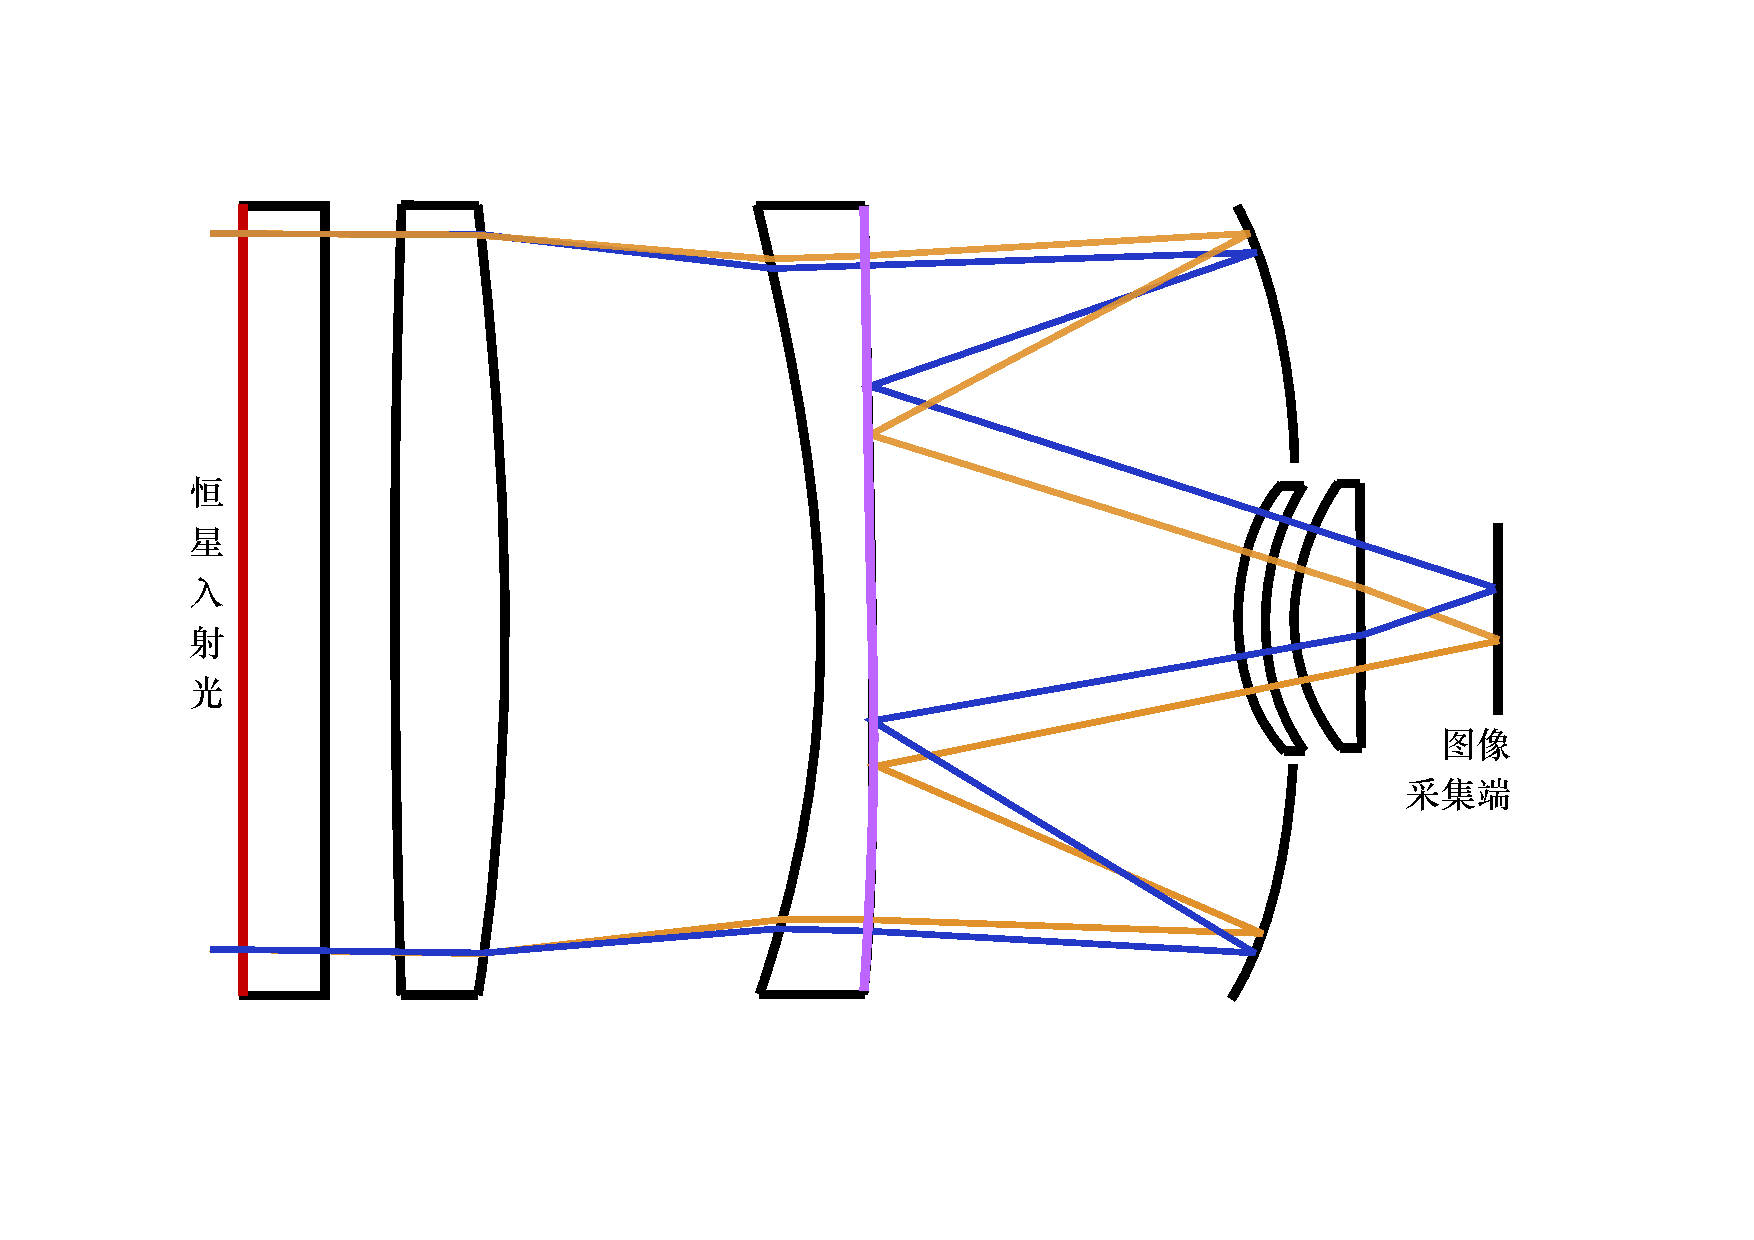
\includegraphics[width=1.0\textwidth]{figures/chapter2/f2_cstaroptics.pdf}
\caption[CSTAR 多镜面结构光路设计图。入射平板镜(最左侧)由改正镜与滤镜组成,最右侧的镜片为中空反射球面镜,中间子镜的右侧面涂有反射材料,该图与实际大小不成比例。]{CSTAR 多镜面结构光路设计图。入射平板镜(最左侧)由改正镜与滤镜组成,最右侧的镜片为中空反射球面镜,中间子镜的右侧面涂有反射材料。作图时未按照实际比例,参考自文献 \citen{ZhouX2010a}。}
\label{fig:cstaroptics}
\end{figure}

CSTAR 于 2008 年 1 月份,正式跟随南极科考队抵达冰穹 A 站点,可惜的是在第一个观测季度结束后,
望远镜只剩下 $i$ 波段镜面能正常观测。于是从 2008 年 3 月 4 日至 8 月 8 日(冰穹 A 站极夜),
CSTAR 共以 20 秒或 30 秒的曝光时间拍摄了超过 310,000 张图片。多亏了极夜创造的连续不间断观测
条件,这些总曝光时间长达 1,728 小时的图片数据表现出良好的科学状况与条件。

随着极昼的到来,科考人员取回了 CSTAR 的原始观测数据,国内两个小组分别开始了独立的分析工
作,国家天文台南极天文小组于 2010 年分别计算了台址当地 $i$ 波段的天光背景以及大气透明度
\cite{Zou2010},并释放出超过 10,000 个恒星点源星表\cite{ZhouX2010b}。Wang 等人\cite{Wang2011}
则于来年在光变数据中找出了 157 颗变星(这高于该天区先前所知数量 6 倍)。随后 Wang 分别在随后
分别对测光给出大气消光、不均匀云层和周天效应的修正(文献 \citen{Wang2012,Wang2014})。

下面,本文将简要介绍文献 \cite{ZhouX2010b} 的主要数据处理流程。在完成扣除本底和平场等预数据
处理后,Zhou 对每张原始图片采用了以 3, 4 和 5 为半径的孔径测光(apeture photometry)。接着,
一张测光条件较好的图被选用作为标准参考,并用模式匹配来认证不同图内相同参考星的位置变化,并
同时矫正其他图片内点源的星等偏差量。以上操作得到标准星表后,其中 48 颗恒星被挑选出来和 
USNO-B1.0 参考星表对比从而得到最终星表。在以上的工作中,作者发现数据中的鬼像修正对于进一步
提高测光精度有着非常重要的意义。

\subsection{鬼像简介以及修正 CSTAR 数据中的鬼像} \label{sec:ghost}

\subsubsection{鬼像以及 CSTAR 中的鬼像}
正如前文(\S \ref{sec:cstardesign})提到,鬼像在光学系统中并不算罕见,尤其是拥有大视场的施密
特望远镜。U.K. 施密特望远镜单元(UKSTU) 将鬼像的产生原因共归为五类,分别是乳化剂涂层、滤
片修正镜、改正镜、滤光片以及尖状鬼像。CSTAR 在设计上采取施密特卡式光学设计,因而鬼像很可
能产生于恒星入射光传播、折射与反射的过程中。UKSTU 手册\cite{1983ukstu} 将此类鬼像定性形容成
弥散状的斑点,且鬼像光斑坐标与产生鬼像的亮源位置关于光学轴对称。对于 CSTAR 而言,鬼像修正
十分必要,因为鬼像不仅会被误认证成一颗恒星源,还会叠加在背景恒星上从而造成额外的测光误差。

\begin{figure}[t]
\centering
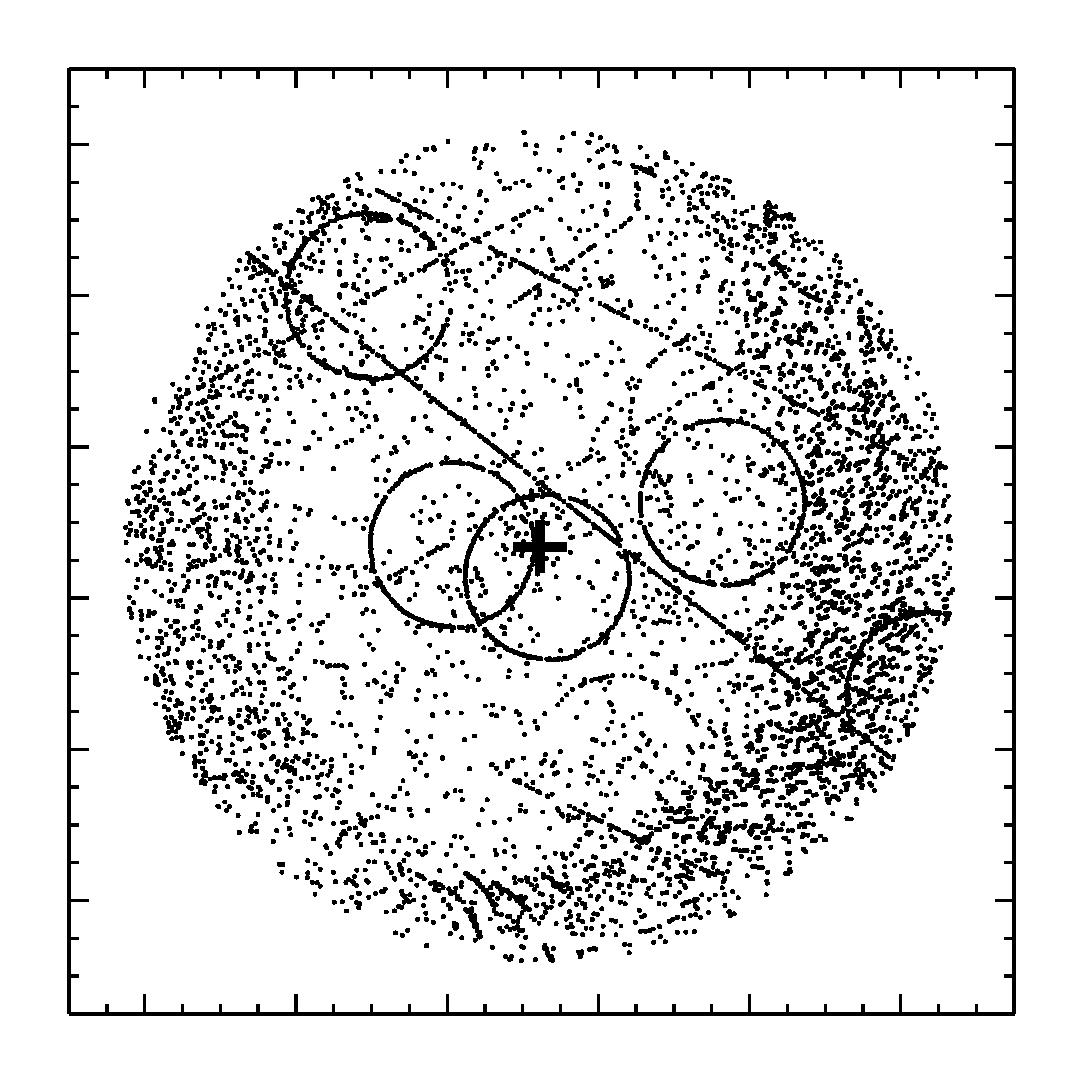
\includegraphics[width=1.0\textwidth]{figures/chapter2/f3_ghoststack.eps}
\caption{周天鬼像叠加图,也即「脏」图。图中的圆弧结构为鬼像所致,黑色十字标注的是南极点。为了更好的看清鬼像的结构,我们已经将已确认的恒星从本图中剔除。}
\label{fig:ghoststack}
\end{figure}

作为第一代南极天文望远镜,CSTAR 采取相对安全的凝视模式 --- 望远镜支撑点固定在冰层上,并
且对准南天极附近的天区观测。当恒星做周日运动时,星象斑也会在 CCD 上绕着南极点做近圆周运
动。若选取图「A5CH5029」作为标准参考图,那么经过恒星图案模式匹配(pattern match)后,其余
所有图相对于标准参考图的旋转角度便可被计算出。从而不同时间测得的图像内相同位置的恒星可被识
别认证。此时将相同恒星的本地坐标(pixel coordinate)通过旋转缩放等操作转化成标准参考图内的坐
标后,便可得到与其对应的主坐标(master coordinate)。从上一段文字中,已经得知鬼像(假恒星)
与产生鬼像的亮星关于光学轴对称,所以当恒星们时时刻刻被匹配上的同时,鬼像却只能经过一个周天
后才能匹配上自己。若把一天之内所有拍摄的图片作叠加,然后将同一颗恒星给抹去后,我们可得到周
天鬼像叠加图(请查阅图 \ref{fig:ghoststack})。从图中可以看出,鬼像的转动方向与周日运动方向相
反,鬼像因此也很可能周期性地「撞」到恒星。当然,如果将南极冰川板块的微弱移动\cite{ZhouX2013}
与恒星自身的运动考虑在内,鬼像很有可能在一天内遭遇到多颗恒星,从而对恒星亮度造成多达约 1.0 
星等的变化(如图 \ref{fig:lcwghost} 与 \ref{fig:ghostseq})。若不小心处理这种变化很可能会被误认为恒
星自身的性质,例如恒星耀斑\cite{Liang2016},因此修正鬼像是后续天体物理研究(如搜寻系外行星
\cite{Wang2014CSTAR} 等)的基础工作。

\begin{figure}[t]
\centering
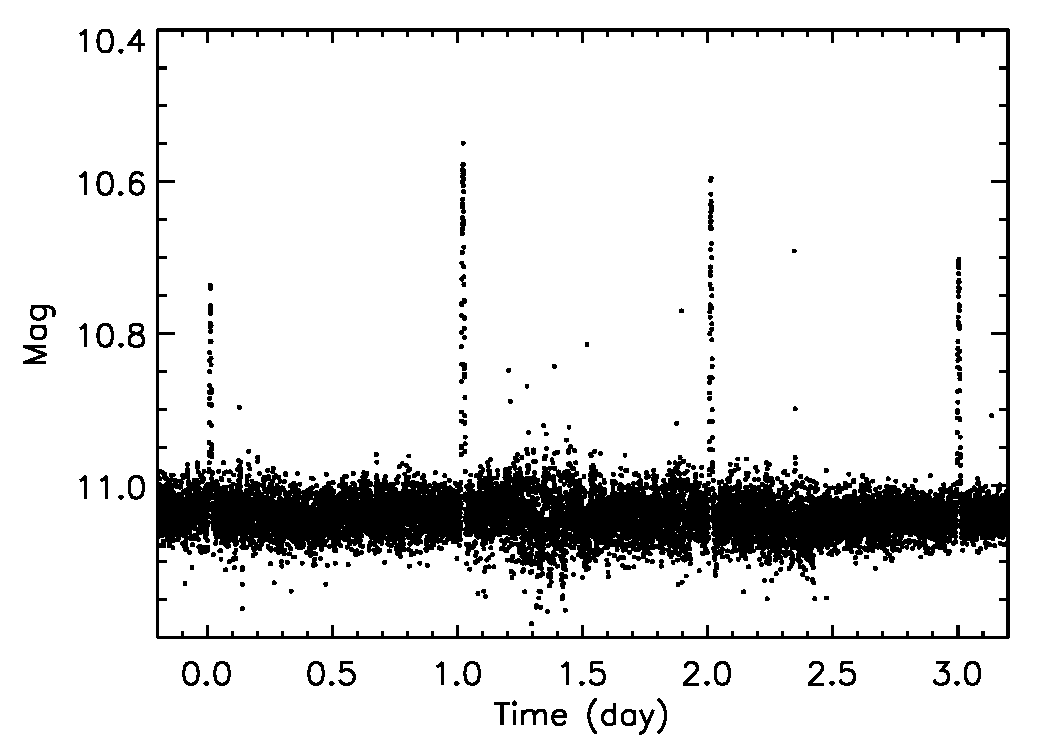
\includegraphics[width=1.0\textwidth]{figures/chapter2/f4_lcwghost.eps}
\caption{CSTAR 视场内坐标为 R.A.: $23^\tif{h}24^\tif{m}28.4^\tif{s}$, decl.: $-89^{\circ}25'10.6''$ 的恒星的光变曲线。通常此特定鬼像会在一个恒星日内遭遇该被影响的恒星一次,从而将恒星的亮度提高半个星等。}
\label{fig:lcwghost}
\end{figure}







\begin{sidewaysfigure}
\centering
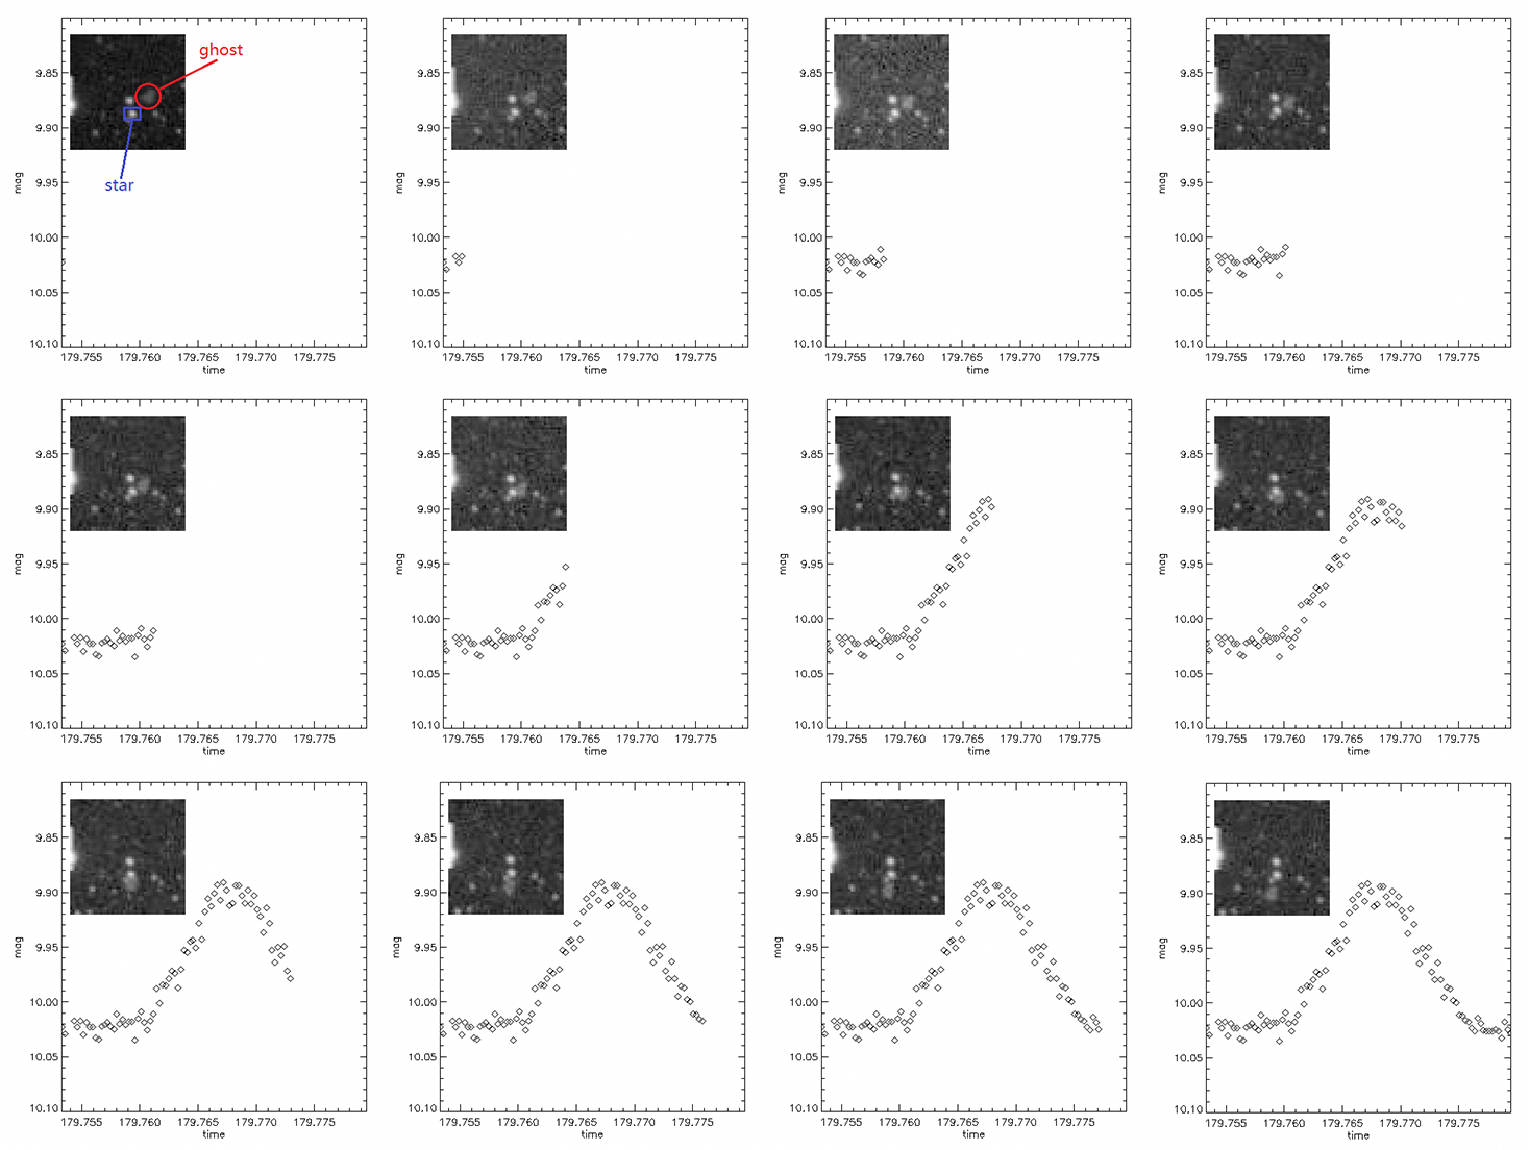
\includegraphics[scale=0.88]{figures/chapter2/f5_ghostseq.pdf}
\caption[坐标相对固定的恒星(蓝色标志)遇到鬼像(红色标注的模糊状弥散源)前后恒星星等的变化程度原始图片数据示意。]{坐标相对固定的恒星(蓝色标志)遇到鬼像(红色标注的模糊状弥散源)前后恒星星等的变化程度原始图片数据示意。每张快照的纵坐标为星等值横坐标为时间,如需查看此图清晰的动画版本请前往网址 \url{https://github.com/meldonization/PhD_Dissertation/blob/master/figures/chapter2/f5_ghostseq.pdf}。}
\label{fig:ghostseq}
\end{sidewaysfigure}


\subsubsection{CSTAR 鬼像修正方法}


\subsubsection{鬼像修正结果及讨论}

\section{AST3 项目中系外行星的巡天策略} \label{sec:ast3}



